% \documentclass[twocolumn]{article}
\documentclass[10pt,conference]{IEEEtran}
%\documentclass[runningheads]{llncs}

\usepackage{babel}
\usepackage{inputenc}
\usepackage{pifont}

%% Math
\usepackage{mathtools}
\usepackage{amsmath}
\usepackage{commath}

\usepackage{amsfonts}% revise se precisa ou não
\usepackage{nccmath}% revise se precisa ou não

\usepackage[numbers]{natbib}
\usepackage{multirow}
\usepackage{makecell}
\usepackage{graphicx}

\usepackage{listings}
\usepackage{float}
\usepackage{enumitem}

\usepackage{wasysym}
\usepackage{resizegather}
\usepackage{rotating}

%\usepackage{caption}
%\captionsetup[table]{skip=5pt}
%\captionsetup[table]{position=above}

\renewcommand{\lstlistingname}{Código}
\renewcommand{\lstlistlistingname}{Lista de \lstlistingname s}

%\definecolor{codegreen}{rgb}{0,0.6,0}
%\definecolor{codegray}{rgb}{0.85,0.85,0.85}
%\definecolor{codepurple}{rgb}{0.58,0,0.82}
%\definecolor{codeblack}{rgb}{0,0,0}

\lstdefinelanguage{JavaScript}{
  keywords={typeof, new, true, false, catch, function, return, null, catch, switch, var, if, in, while, do, else, case, break},
  %keywordstyle=\color{blue}\bfseries,
  ndkeywords={class, export, boolean, throw, implements, import, this},
  %ndkeywordstyle=\color{codegray}\bfseries,
  %identifierstyle=\color{black},
  sensitive=false,
  comment=[l]{//},
  morecomment=[s]{/*}{*/},
  %commentstyle=\color{purple}\ttfamily,
  %stringstyle=\color{red}\ttfamily,
  morestring=[b]',
  morestring=[b]"
}

\lstdefinestyle{codigo}{
    backgroundcolor=\color{codegray},   
    commentstyle=\color{codegreen},
    keywordstyle=\color{magenta},
    numberstyle=\tiny\color{codeblack},
    stringstyle=\color{codepurple},
    basicstyle=\ttfamily\footnotesize,
    breakatwhitespace=false,         
    breaklines=true,                 
    captionpos=b,                    
    keepspaces=true,                 
    numbers=left,                    
    numbersep=5pt,                  
    showspaces=false,                
    showstringspaces=false,
    showtabs=false,                  
    tabsize=4
}

\lstset{style=codigo}

\DeclarePairedDelimiter{\round}\lfloor\rceil
\newcommand\citetxt[1]{%
  \citeauthor{#1}~(\citeyear{#1})}
\newcommand\citepar[1]{%
  (\citeauthor{#1}, \citeyear{#1})} 
  


%https://tex.stackexchange.com/q/151984/7561
\DeclarePairedDelimiterX{\infdivx}[2]{(}{)}{%
  #1\;\delimsize\|\;#2%
}
\newcommand{\kl}{\operatorname{KL}\infdivx}
\newcommand{\skl}{\operatorname{SKL}\infdivx}

% https://tex.stackexchange.com/questions/23773/a-centered-plus-minus-symbol
\newcommand{\rpm}{\raisebox{.2ex}{$\scriptstyle\pm$}}

% https://tex.stackexchange.com/a/141685/7561
\newcommand\givenbase[1][]{\:#1\lvert\:}
\let\given\givenbase

% https://tex.stackexchange.com/a/171959/7561
\newcommand\reallywidehat[1]{\ThisStyle{%
    \setbox0=\hbox{$\SavedStyle#1$}%
    \stackengine{-1.0\ht0+.5pt}{$\SavedStyle#1$}{%
      \stretchto{\scaleto{\SavedStyle\mkern.15mu\char'136}{1.5\wd0}}{1.4\ht0}%
    }{O}{c}{F}{T}{S}%
}}
\newcommand{\hkl}{\widehat{\operatorname{KL}}\infdivx}

% Conditional independence symbol
% https://tex.stackexchange.com/questions/218631/symbol-for-not-conditionally-independent/
\newcommand{\CI}{\mathrel{\perp\mspace{-10mu}\perp}}

% declare my argmin and argmax operators
% https://tex.stackexchange.com/a/5255/7561
\DeclareMathOperator*{\argmax}{arg\,max}
\DeclareMathOperator*{\argmin}{arg\,min}

% declaring an expectation operator to behave like sum
% https://tex.stackexchange.com/a/23436/7561
\makeatletter
\DeclareRobustCommand\bigop[1]{%
  \mathop{\vphantom{\sum}\mathpalette\bigop@{#1}}\slimits@
}
\newcommand{\bigop@}[2]{%
  \vcenter{%
    \sbox\z@{$#1\sum$}%
    \hbox{\resizebox{\ifx#1\displaystyle.9\fi\dimexpr\ht\z@+\dp\z@}{!}{$\m@th#2$}}%
  }%
}
\makeatother

% Keywords command
\providecommand{\keywords}[1]
{
  \small	
  \textbf{\textit{Keywords ---}} #1
}
\providecommand{\palavraschave}[1]
{
  \small	
  \textbf{\textit{Palavras-chave ---}} #1
}

%\newcommand{\E}{\DOTSB\bigop{\mathbb{E}}}
\DeclareMathOperator*{\E}{\mathbb{E}}

% redefining \times operator
\let\oldtimes\times
\def\times{{\mkern1mu\oldtimes\mkern1mu}}



\usepackage{subfigure}
\newcommand{\cmark}{\ding{51}}%

%\DeclarePairedDelimiter\abs{\lvert}{\rvert}%
%\DeclarePairedDelimiter\norm{\lVert}{\rVert}%
\DeclarePairedDelimiter\product{\langle}{\rangle}%

\usepackage{cellspace}
\setlength\cellspacetoplimit{6pt}
\setlength\cellspacebottomlimit{4pt}

%% Units
\usepackage{siunitx}

%% Tables
\usepackage{booktabs}


% Para acrescentar comentários ao PDF descomente:
\usepackage
%  [pdfauthor={nome do autor},
%   pdftitle={titulo},
%   pdfkeywords={palavra-chave, palavra-chave},
%   pdfproducer={Latex with hyperref},
%   pdfcreator={pdflatex}]
{hyperref}

% Os cores podem ser mudados
\hypersetup{
%  linkcolor={red!50!black},
%  citecolor={blue!50!black},
%  urlcolor={blue!80!black}
}

\usepackage{url}
\usepackage{breakurl}
% \usepackage[breaklinks]{hyperref}

\def\UrlBreaks{\do\/\do-\do\_}

\title{A semi-autonomic solution for developing Machine Learning-based applications using Fairness metrics}
%\titlerunning{Semi-autonomic Workflow for ML applications using \textit{Fairness} metrics}


%\author{Thales Eduardo Nazatto\textsuperscript{1}, Cecília Mary Fischer Rubira\textsuperscript{2}, Leonardo Montecchi\textsuperscript{3}}
%\authorrunning{Thales Eduardo Nazatto, Cecília Mary Fischer Rubira, Leonardo Montecchi}
%\author{
%	\IEEEauthorblockN{Thales Eduardo Nazatto}
%	\IEEEauthorblockA{
%		UNICAMP, Campinas, Brazil \\
%		tenazatto@gmail.com}
%	\and
%	\IEEEauthorblockN{Cecília Mary Fischer Rubira}
%	\IEEEauthorblockA{
%		UNICAMP, Campinas, Brazil \\
%		cmrubira@ic.unicamp.br}
%	\and
%	\IEEEauthorblockN{Leonardo Montecchi}
%	\IEEEauthorblockA{
%		NTNU, Trondheim, Norway \\
%		leonardo.montecchi@ntnu.no}
%}

%\date{
%	\textsuperscript{1} UNICAMP, Campinas, Brazil, tenazatto@gmail.com
%	\\
%	\textsuperscript{2} UNICAMP, Campinas, Brazil, cmrubira@ic.unicamp.br
%	\\
%	\textsuperscript{3} NTNU, Trondheim, Norway, leonardo.montecchi@ntnu.no\\[2ex]
%	\today
%}

%\institute{
%	\textsuperscript{1} UNICAMP, Campinas, Brazil, tenazatto@gmail.com
%	\\
%	\textsuperscript{2} UNICAMP, Campinas, Brazil, cmrubira@ic.unicamp.br
%	\\
%	\textsuperscript{3} NTNU, Trondheim, Norway, leonardo.montecchi@ntnu.no\\[2ex]
%}

\begin{document}

\maketitle

\begin{abstract}
Machine Learning (ML) is increasingly used with big data to make faster and more assertive decisions, but initial metrics to evaluate algorithms have proven limited in measuring biases that reflect society in an unexpected way. To address this, new Fairness algorithms and metrics have been created to balance discriminated groups, but it increases the complexity for Data Scientists to develop the best models. This article focuses on Machine Learning solutions from a Software Engineering point of view, presenting a Workflow that uses the MAPE-K architecture to determine which algorithm has the best balance, without having to test many techniques. Several case studies were carried out to verify the feasibility of MAPE-K in solving problems, and if the solution can be easily extended to allow the use of more algorithms. This can help ML Specialists to do Software Engineering studies on applications with responsible use of data.

\keywords{Automated Machine Learning, AI Ethics, Social Responsibility in AI, Autonomic Loop, Fairness metrics, MAPE-K}
\end{abstract}

\section{Introduction}

Artificial Intelligence (AI) and Machine Learning (ML) techniques have been used for a long time in the field of Computer Science. Areas such as robotics and games are great examples, given their need to automate behaviors that would be considered trivial for a human being. However, in recent years there has been a growth in the use of these technologies in traditional applications, mainly due to the large amount of data processed daily by companies and the amount of processing available at low costs. Different profiles can be drawn from these data and using AI solutions generate more assertive decision making in order to improve the user experience and correct problems. However, a common side effect in these solutions is the exposure of biases that, although seen as unintentional by developers due to the possibility of being an \textit{outlier} in the trained model, reflect open prejudices of today's society. Biased data entries result in an algorithm that performs discriminations in its classification~\citep{Buolamwini_2018}, and since the metrics used to measure the quality of final model are generally based on accuracy, precision and recall, social contexts and discrimination are not easily perceived by such metrics.

Due to this problem, it is possible to establish different metrics to determine how well the model is prepared for sensitive data~\citep{Begley_2021}, a term that is known as \textit{Fairness}. With the evolution of academic research on this concept, new methods were defined to reduce the biases present in datasets, such as \textit{Reweighing}~\citep{Kamiran_2011}, \textit{Adversarial Debiasing}~\citep{Zhang_2018} and \textit {Reject Option Classification}~\citep{Kamiran_2012}. Consequently, there is an improvement in these metrics, but it may disfavor metrics that are already widely used as a guarantee of an effective model developed with Machine Learning techniques.

For this particular context, a method for developing Machine Learning applications was developed, which is handled by Data Scientists in a semi-autonomous way, focused on two main objectives:

\begin{itemize}
\item Make the creation of fair and reliable models by automating the choice of algorithms easier, due to increased complexity in choosing algorithms to be used and their execution in the correct steps of the process.
\item Define a balance between metrics for evaluating good models with metrics for evaluating fair models.
\end{itemize}

This structure is divided into 5 modules: Data Engineering, ML Workflow, Autonomic Manager, Backend and Frontend. For Data Engineering, modifications were made to the German Credit Dataset~\citep{ucigerman_2021} and Lendingclub Dataset~\citep{lendingclub_2022} datasets to be suitable for the \textit{workflow} implementation. For the workflow development, the \textit{Pipes-and-Filters} architecture was used. For the Autonomic Manager, the MAPE-K~\citep{IBM_2005} architecture was used to analyze a knowledge base and provide the best configuration background following predetermined rules. For the Frontend and the Backend, its creation was thought of a web application template\footnote{Repository containing the codes for this project: \url{https://anonymous.4open.science/r/FAIR-2EFD}} for evaluation and testing in further studies.

\section{Background}

\subsection{Autonomic Computing}

In 2001, Paul Horn introduced the concept of Autonomic Computing as a possible solution to the growing complexity of systems at the time, where it was predicted that they would become too large and complex for even the most qualified professionals to configure and maintain. This concept qualifies computing systems that can self-manage in relation to the high-level goals given by administrators and is derived from biology, given the great variety and hierarchy of autonomous systems existant in nature and society~\citep{Kephart_2003}.

To Autonomic Computing works as intended, an Autonomic Element~\citep{Abbas_2010} is implemented, a software component that manages parts of the system based on a \textit{loop} MAPE-K (\textit{Monitor, Analyze, Plan, Execute, and Knowledge}), illustrated in Figure \ref{fig:MAPEK}. MAPE-K is a concept that constitutes a control \textit{loop}, used to monitor and control one or more Managed Elements. A Managed Element can be hardware such as a printer, software such as a database, another Autonomous Element, or specific functions such as load balancing. A MAPE-K control \textit{loop} is split as follows:

\begin{itemize}
\item \textbf{Monitor:} Responsible for monitoring managed resources and collecting, aggregating and filtering data. Monitoring is done through one Sensor or more.
\item \textbf{Analyze:} Analyzes the data reported by the monitor part. The analysis aims to understand what the current state of the system is and if there are measures to be taken.
\item \textbf{Plan:} An action plan is prepared in the basis of the analysis' results. The plan is a series of measures that will move the system from its current state to a desired state.
\item \textbf{Execute:} The plan is executed and controlled. One Effector or more perform the planned actions on the resource.
\item \textbf{Knowledge:} The knowledge base is central and accessible by all parts of the \textit{loop}. Separated from collected and analyzed data, it contains additional knowledge such as architectural models, goal models, policies and change plans.
\end{itemize}

\begin{figure}[H]
\centering
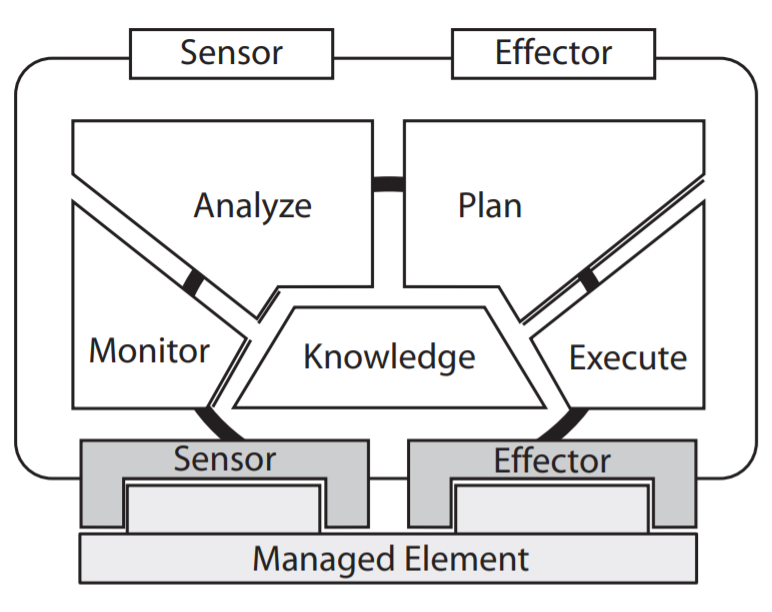
\includegraphics[scale=0.5]{images/MAPE-K.png}
\caption {MAPE-K architecture diagram~\citep{Abbas_2010}.}
\label{fig:MAPEK}
\end{figure}

\subsection{Machine Learning}
Machine Learning can be defined as “the practice of using algorithms to collect data, learn from it, and then make a determination or prediction about something in the world. Instead of manually implementing code to complete a particular task, the machine is `trained` using large amount of data and algorithms that give it the ability to learn how to perform tasks.

The method for training a machine are composed by the following steps:

\begin{itemize}
\item Data collection
\item Data cleaning and refinement
\item Data preparation and split into training and test sets
\item Algorithm training and learning using the training set
\item Metric evaluation using the test set
\end{itemize}

A Machine Learning algorithm can be classified into three basic categories:

\begin{itemize}
\item \textbf{Supervised learning}: Training is performed using labeled examples, such as an input in which the desired output is known. Through methods such as classification, regression, and \textit{gradient boosting}, supervised learning uses patterns to predict the values of labels in additional unlabeled data. Supervised learning is commonly employed in applications where historical data predict likely future events.
\item \textbf{Unsupervised Learning}: Used on data that does not have historical labels. The “right answer” is not reported to the system, the algorithm must figure out what is being shown. The goal is to explore the data and find some structure within it. Popular techniques include self-organizing maps, proximity mapping, \textit{k-means}, and singular value decomposition. These algorithms are also used to segment text topics, recommend items, and identify outliers in data.
\item \textbf{Reinforcement learning}: The algorithm discovers through trial-and-error testing which actions yield the greatest rewards. This type of learning has three main components: the agent (the learner or decision maker), the environment (everything the agent interacts with) and actions (what the agent can do). The objective is for the agent to choose actions that maximize the expected reward in a given period of time. The agent will reach the goal much faster if it follows a good policy, so the focus of reinforcement learning is to discover the best policy.
\end{itemize}

\subsection{\textit{Fairness} in Machine Learning}

\begin{figure*}[h]
\centering
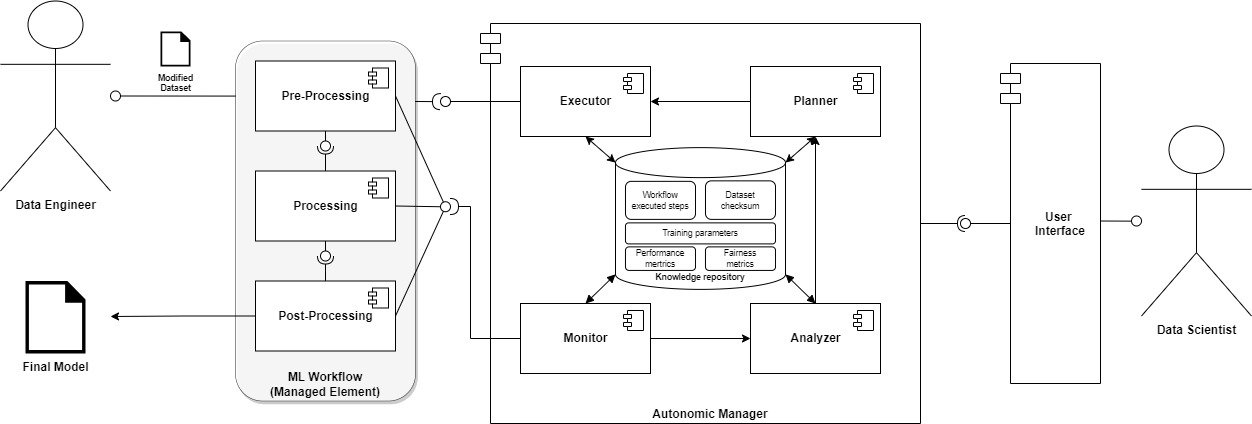
\includegraphics[scale=0.4]{images/backend-frontend-ml-eng.jpg}
\caption {Architecture components of the proposed solution}
\label{fig:BackendFrontendML}
\end{figure*}

It is possible to describe the concept of \textit{Fairness} in the context of supervised learning, where a model $f$ can predict a set of results $y$ from a set of \textit{features} $x$, avoiding unfair discrimination against a protected attribute $a$. It is allowed, but not required, for $a$ to be a component of $x$~\citep{Begley_2021}. In other words, a fair ML model is one where the correlation of its result is low in relation to input data considered sensitive to discrimination. Machine Learning algorithms are not able to differentiate social contexts, where a more efficient result according to the available data can amplify social inequalities and make decisions unfairly~\citep{Mehrabi_2021}. These sensitive data, such as race, sex, age and height, are considered protected attributes, which need to be classified and processed before the execution of a Machine Learning algorithm, which will determine how the algorithm will behave and, consequently, will affect the metrics~\citep{Mougan_2022}. The groups of data from these protected attributes are considered protected groups, which can be divided into two groups: the privileged group, which has advantages in the problem's context, and the non-privileged group, which has disadvantages in the problem's context and, therefore, subject to discrimination.

Fairness metrics differ from the metrics used for model evaluation, which have the purpose of checking whether a model has reliable predictions or not. While the more traditional metrics evaluate the performance of the model, data as a whole and general results, Fairness metrics evaluate whether the general results are also reflected in specific groups, to verify that there is no disparity or discrimination in the proposed results. Examples of metrics used for this are Statistical Parity Difference, or discrimination~\citep{Zemel_2013}, Equal Opportunity Difference~\citep{Biswas_2020}, Average Odds Difference~\citep{Biswas_2020}, Disparate Impact~\citep{Biswas_2020} and Theil Index~\citep{Speicher_2018}. Almost all of these metrics needs a value close to 0 to be considered fair. The only exception is Disparate Impact which needs a value close to 1 due to the fact this metric is the only one which is calculated as a ratio.

To balance these metrics in a ML model, new algorithms were created to make the learning process more prepared to deal with biased data, which can be classified into three categories: 

\begin{itemize}
\item \textbf{Pre-processing:} These algorithms try to remove discrimination by transforming the data. Some examples are \textit{Disparate Impact Remover}~\citep{Feldman_2015}, \textit{Learning Fair Representations}~\citep{Zemel_2013}, \textit{Reweighing}~\citep{Kamiran_2011} and \textit{Optimized Preprocessing}~\citep{Calmon_2017}
\item \textbf{Processing:} These algorithms try to mitigate discrimination during the training process. Some examples are \textit{Adversarial Debiasing}~\citep{Zhang_2018}, \textit{Exponentiated Gradient Reduction}~\citep{Agarwal_2018}, \textit{Grid Search Reduction}~\citep{Agarwal_2019}, \textit{Meta Fair Classifier}~\citep{Celis_2019}, \textit{Prejudice Remover}~\citep{Kamishima_2012} and \textit{Rich Subgroup Fairness}~\citep{Kearns_2018}
\item \textbf{Post-processing:} These algorithms change the predictions made by an already trained model to make it fair. Some examples are \textit{Equalized Odds}~\citep{Hardt_2016}, \textit{Calibrated Equalized Odds}~\citep{Pleiss_2017} and \textit{Reject Option Classification}~\citep{Kamiran_2012}.
\end{itemize}

\section{The Proposed Solution}

\subsection{Architecture and Implementation}

%\begin{figure*}[h]
%\centering
%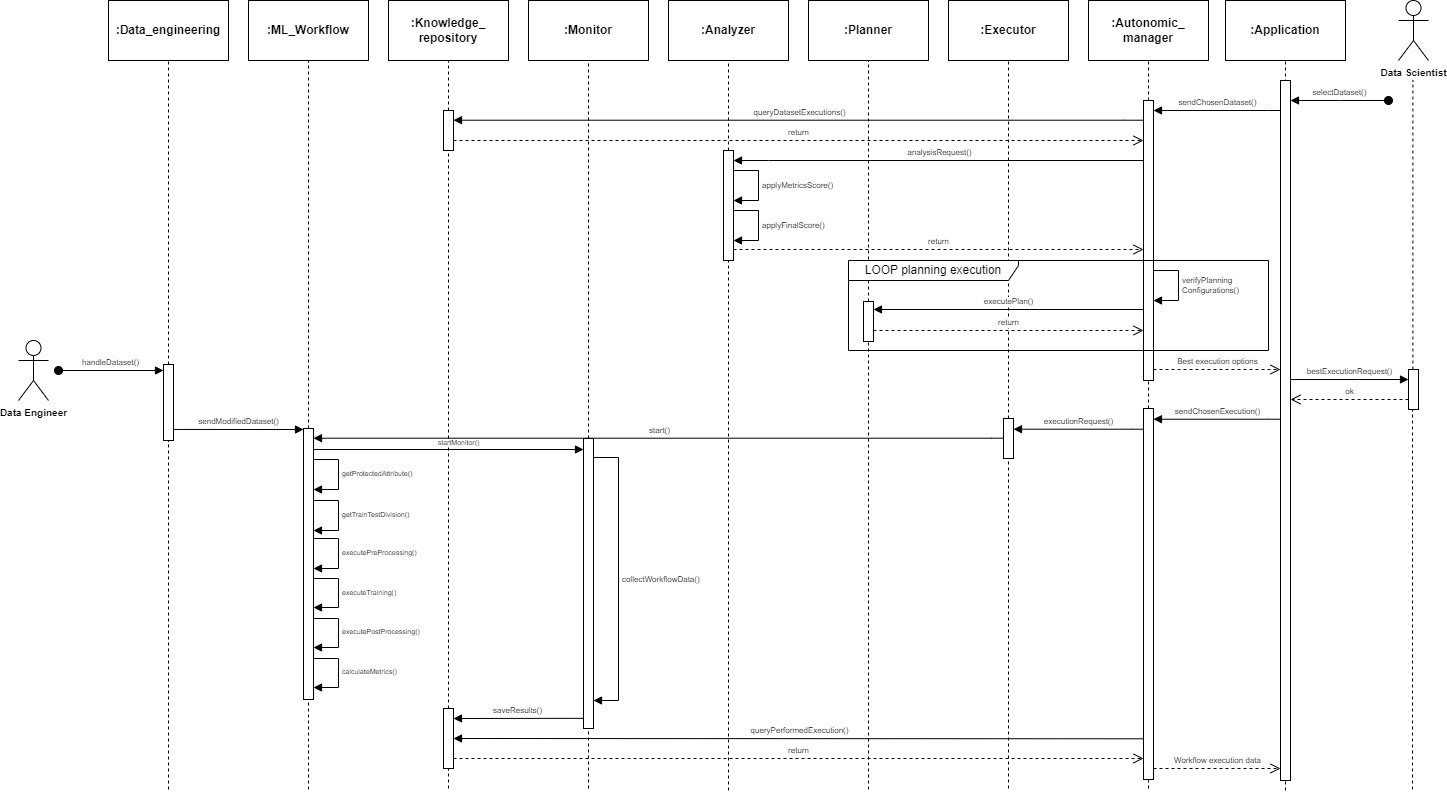
\includegraphics[scale=0.35]{images/Diagrama_Sequencia-eng.jpg}
%\caption {System's sequence diagram}
%\label{fig:DiagramaSequencia}
%\end{figure*}
\begin{sidewaysfigure*}
\clearpage
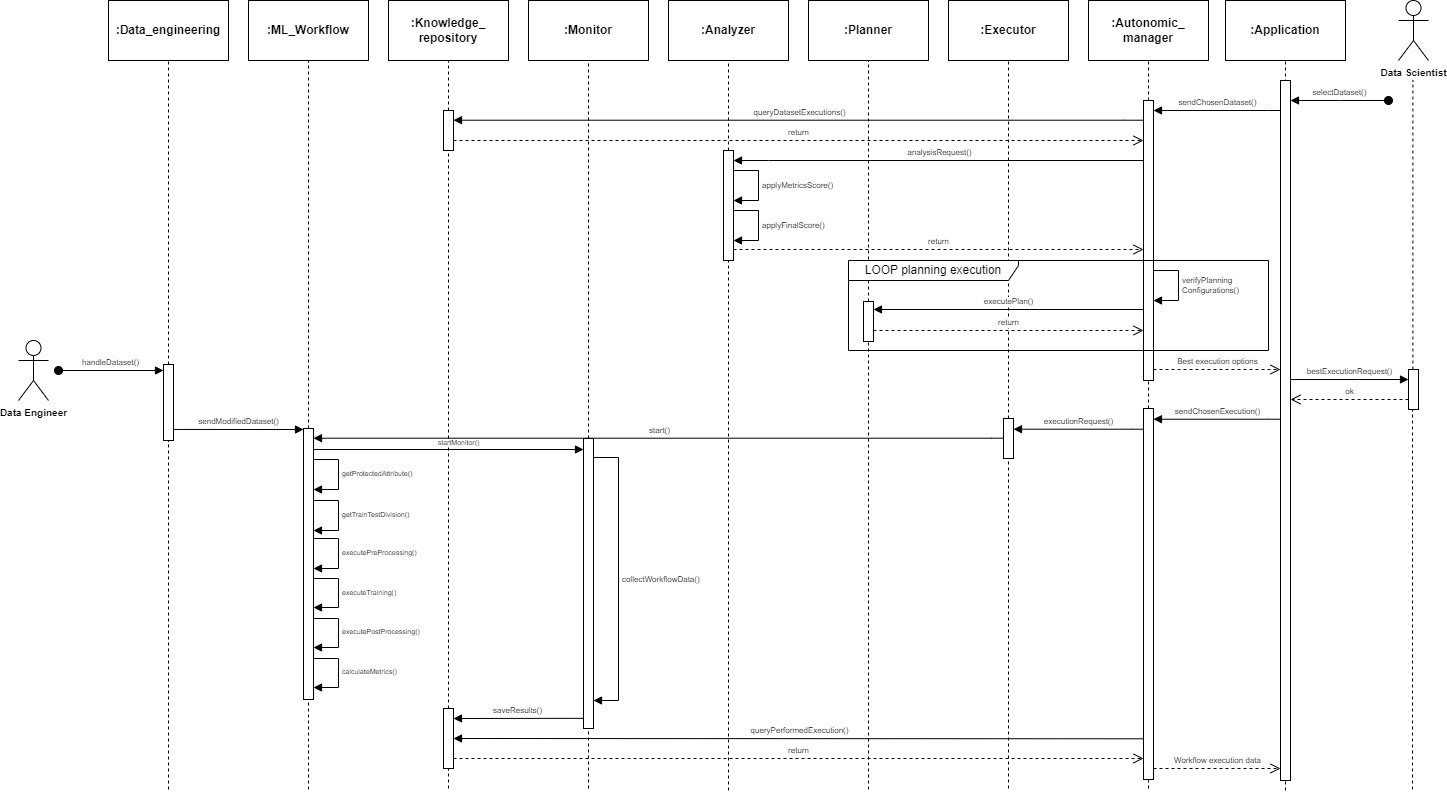
\includegraphics[scale=0.465]{images/Diagrama_Sequencia-eng.jpg}
\caption {System's sequence diagram}
\label{fig:DiagramaSequencia}
\end{sidewaysfigure*}

The solution architecture is divided into 5 modules:

\begin{itemize}
    \item {\textbf{Data Engineering:}} Module with the objective of executing data transformation and cleaning processes.
	\item {\textbf{ML Workflow:}} Module that executes a Pipeline of an automated ML application, with stages of data preparation (Pre-processing), training (Processing) and result evaluation (Post-processing) of the final model generation.
     \item {\textbf{Autonomic Manager:}} Module containing a MAPE-K \textit{loop} that controls the Workflow as a Managed Element to automate all its steps, in order to avoid manual executions depending on the algorithm and/or dataset used on the stages.
     \item {\textbf{User Interface (Frontend):}} Module which goal is to provide a simpler and more intuitive user experience for the Data Scientist in order to configure and start the Autonomic Manager.
	\item {\textbf{Backend:}} Module created with the objective of connecting the Frontend to the Autonomic Manager.
\end{itemize}

The integration between these modules is illustrated in Figure \ref{fig:BackendFrontendML}. The Data Engineering module is used by the Data Engineer, who would return a dataset with the necessary treatments for execution within the supervised learning workflow. The Frontend module would be used by the Data Scientist, who would determine the settings needed to choose the configuration background depending on the problem's context. 

The process that takes place, from the User Interface interaction, passing through the execution of workflow and finishing at obtaining the results, can be visualized in the Sequence Diagram present in Figure \ref{fig:DiagramaSequencia}. In this process, while the Data Engineer handles the dataset with transformation and cleaning processes presented in the Data Engineering module and send the modified datasets to integrate and use into ML Workflow, the Data Scientist, via the application's User Interface, choose the dataset and demand an Autonomic Manager execution. The Autonomic Manager queries all the executions made by the ML Workflow that used this dataset and are saved into the Knowledge Repository, do the analysis making some calculations that will be detailed in the next sections, and do a loop verifying the configuration of some implemented execution plans and executing them, returning some best execution options and wait the Data Scientist evaluation to choose one option to request a new ML Workflow execution. After the request, the ML Workflow starts the Monitor to collect data during its execution, get the chosen dataset and protected attribute, split into training and test sets, execute the chosen algorithms in the Pre-processing, Processing and Post-processing steps, and calculate the final model metrics. The Monitor save all collected data into the Knowledge Repository, and the Autonomic Manager queries this performed execution data to show to the Data Scientist.

\subsection{Monitor and Analysis Component behavior}

To guarantee the workflow autonomy, the Monitor component collects the data obtained during a execution (metrics, parameters and executed steps) and organizes them for the Analyzer to make the data analysis process. In this process, a calculation of weights based on specific metrics is performed to consolidate all metrics and simplify planning strategies. Metrics are divided into two groups (Performance metrics and Fairness metrics), and within this group you can place as many metrics as necessary, as long as the context of each group is respected. Each group is assigned different weights, and each metric in that group is also assigned different weights. The reason these weights exist in the calculation is to give a measure of the problem's context, according to a prior analysis by the Data Scientist and Domain Specialist.

First, it is necessary to standardize the Fairness metrics $m_{F_i}$ to $m'_{F_i}$ in an interval from 0 to 1, as presented in Equation \ref{eqn:normalizationFairness}. This guarantees the result consistency and the correct application of weights, avoiding distortions in the calculation. As Fairness metrics can involve both the ratio between two different values, like \textit{Disparate Impact}, and the difference between two different values, like \textit{Equal Opportunity Difference}, different calculations are required to get that range. As the evaluated Performance metrics have the same range from 0 to 1, there is no need for additional treatment for the metrics $m_{P_i}$.

Then, each standardized metric is multiplied by its corresponding weights $w_{P_i}$ and $w_{F_i}$, and a weighted average is taken within the group to assign a score $S_P$ to the Performance metrics group and $S_F$ for the Fairness metrics group, as shown in equation \ref{eqn:groupScores}. To make the score evaluation easier, the scores are multiplied by a factor $X = 1000$ to make the score range is 0 to 1000 and the value is rounded. After such scores are obtained, the overall score $S$ is calculated by multiplying them by their corresponding weights $w_P$ and $w_F$ and arranging the weighted average as shown in equation \ref{eqn:totalScore}.

\begin{gather}
\label{eqn:normalizationFairness}
	m'_{F_i} = 
	\begin{cases}
	1-\lvert m_{F_i} \rvert & \text{if $m_{F_i}$ is subtraction-calculated and $-1 < m_{F_i} < 1$}\\
	0 & \text{if $m_{F_i}$ is subtraction-calculated, and $m_{F_i} >= 1$ or $m_{F_i} <= -1$}\\
	1-\lvert \frac{1}{m_{F_i}}-1 \lvert & \text{if $m_{F_i}$ is division-calculated and $m_{F_i} > 1$}\\
	1-\lvert m_{F_i}-1 \lvert & \text{if $m_{F_i}$ is division-calculated e $m_{F_i} <= 1$}\\
	m_{F_i} & \text{in other cases}
	\end{cases}
\end{gather}

\begin{equation}
\label{eqn:groupScores}
	\begin{aligned}
	S_F = \round{X \times \frac{\sum_{i=1}^{n_F} w_{m'_{F_i}} \times m'_{F_i}}{\sum_{i=1}^{n} w_{m'_{F_i}}}}\\
	S_P = \round{X \times \frac{\sum_{i=1}^{n_P} w_{m_{P_i}} \times m_{P_i}}{\sum_{i=1}^{n} w_{m_{P_i}}}}
	\end{aligned}
\end{equation}

\begin{equation}
\label{eqn:totalScore}
	S = \frac{w_F \times S_F + w_P \times S_P}{w_F + w_P}
\end{equation}

To do these calculations, previous executions in the workflow are needed as a prerequisite, so the necessary metrics could be recorded and then the best combinations are determined through the score.

\subsection{Planner Component}

To determine the configuration background, some strategies were implemented in the Planner component:

\begin{itemize}
\item \textbf{Algorithm filtering}: Some algorithms may be poorly implemented on Workflow or their models may have metrics that need a better analysis by the Data Scientist to be considered reliable. To prevent this from happening, this strategy filters reliable algorithm combinations before selecting the ideal models.
\item \textbf{Result range}: Executions with unreliable metric results can distort the score obtained in the Analyzer. To ease these distortions, a minimum and maximum score range were created to determine scores that can be considered reliable for evaluation.
\end{itemize}

After evaluating these strategies, the Planner component will return the top 5 scores for the Data Scientist to choose, and will ask the Executor to run the Workflow again after choosing.

\section{Solution Evaluation}

Three Case Studies were executed to check our solution feasibility, future maintenance and the Autonomic Manager feasibility in choosing the best options in different contexts. In all of them, the objective was to obtain a credit rating (good or bad), through a series of \textit{features} and using different datasets. In the case of system changes, the lines of code performed in each change were also counted, to define whether such changes are simple to make.

The execution to choose the best options was performed with 3 different weightings in the overall score:

\begin{itemize}
\item 50\% for Performance metrics and 50\% for Fairness metrics, for a balanced setup.
\item 75\% for Performance metrics and 25\% for Fairness metrics, for a configuration that prioritizes performance over fairness.
\item 25\% for Performance metrics and 75\% for Fairness metrics, for a configuration that prioritizes fairness over performance.
\end{itemize}

All executions were performed using a knowledge base containing about 650 previous executions with several options of datasets, protected attributes and algorithms, containing in your results the metrics Accuracy, Precision, Recall, F1-Score and AUC as Performance metrics and the metrics Statistical Parity Difference, Equal Opportunity Difference, Average Odds Difference, Disparate Impact and Theil Index as Fairness metrics. All metrics have the same weight in their respective grouping.

In the workflow, the algorithms \textit{Disparate Impact Remover}, \textit{Learning Fair Representations}, \textit{Reweighing} and \textit{Optimized Preprocessing} were implemented in the Pre-Processing step, the algorithms Logistic Regression, Gradient Boosting, Random Forest, Support Vector Machines, \textit{Adversarial Debiasing}, \textit{Exponentiated Gradient Reduction}, \textit{Grid Search Reduction}, \textit{Meta Fair Classifier}, \textit{Prejudice Remover} and \textit{Rich Subgroup Fairness} were implemented in the Processing step, and the algorithms \textit{Equalized Odds}, \textit{Calibrated Equalized Odds} and \textit{Reject Option Classification} were implemented in the Post-Processing step. As no studies were found where bias reduction is used in more than one step of the Machine Learning process only one bias reduction algorithm per workflow is performed in a execution. Due to unreliable data, executions with the algorithms \textit{Optimized Preprocessing} and \textit{Reject Option Classification} were filtered, corresponding to approximately 5\% of total base size.

\subsection{Case Study 1: Autonomic Manager feasibility and usefulness}

In this Case Study, the focus was on testing and verifying how the Autonomic Manager behaves, using the German Credit Dataset~\citep{ucigerman_2021} as the dataset, Age and Nationality as the protected attribute options and a score range between 500 and 950. The results are presented below in the Tables \ref{tbl:ScoreMAPEKOverall5050}, \ref{tbl:ScoreMAPEKOverall7525} and \ref{tbl:ScoreMAPEKOverall2575}.

In these executions, two observations are surprising. The first is the predominant use of post-processing algorithms, especially in settings that prioritized performance, against the expectation that algorithms with bias reduction increased justice at the expense of performance. The second is the predominance of pre-processing algorithms combined with Support Vector Machines as a training algorithm in configurations that prioritized fairness.
In all executions, it was possible to perceive that the most balanced choice between these two groups of metrics with completely different contexts still becomes diffuse in view of the large number of metrics and algorithms used. Furthermore, the difference between the metrics is extremely small and makes the choice even more difficult. In this context, the consolidation of metrics into groups simplifies the visualization of which workflows are more balanced, and the use of weights for each metric and each group could be calibrated with the best desired balance for a given situation. Thus, it can also be concluded that, in a development context, the process simplifies Data Scientist's decision and significantly reduces time to obtain and deploy an optimized model, since it will not require executions in several algorithms since there is a prior knowledge base. In addition, there could be processing and cost savings in case of future problems using the same dataset, since the executions saved by the teams that would use this process make room for other teams to use past data to verify better choices.

\begin{table}[H]
\begin{center}
  \caption{Top options chosen by Autonomic Manager \\ 50\% Performance/50\% Fairness}
\label{tbl:ScoreMAPEKOverall5050}
  \resizebox{\linewidth}{!}{%
\begin{tabular}{c|c|c|c|c|c|c}
\multicolumn{4}{c|}{Workflow} & \multicolumn{3}{c}{Score} \\
\hline
Protected attribute & Pre-processing & Processing & Post-processing & Performance & Fairness & \textbf{Overall} \\
\hline
Age & Nothing & Logistic Regression & Equalized Odds & 968 & 860 & \textbf{914} \\
Nationality & Nothing & Random Forest & Calibrated Equalized Odds & 902 & 922 & \textbf{912} \\
Nationality & Nothing & Gradient Boosting & Calibrated Equalized Odds & 870 & 925 & \textbf{898} \\
Age & Nothing & Gradient Boosting & Equalized Odds & 927 & 862 & \textbf{894} \\
Age & Reweighing & Gradient Boosting & Nothing & 804 & 931 & \textbf{868} \\
\end{tabular}}
\end{center}
\end{table}

\begin{table}[H]
\begin{center}
  \caption{Top options chosen by Autonomic Manager \\ 75\% Performance/25\% Fairness}
\label{tbl:ScoreMAPEKOverall7525}
  \resizebox{\linewidth}{!}{%
\begin{tabular}{c|c|c|c|c|c|c}
\multicolumn{4}{c|}{Workflow} & \multicolumn{3}{c}{Score} \\
\hline
Protected attribute & Pre-processing & Processing & Post-processing & Performance & Fairness & \textbf{Overall} \\
\hline
Age & Nothing & Logistic Regression & Equalized Odds & 968 & 860 & \textbf{941} \\
Age & Nothing & Gradient Boosting & Equalized Odds & 927 & 862 & \textbf{910} \\
Nationality & Nothing & Random Forest & Calibrated Equalized Odds & 902 & 922 & \textbf{907} \\
Nationality & Nothing & Gradient Boosting & Calibrated Equalized Odds & 870 & 925 & \textbf{883} \\
Age & Nothing & Random Forest & Equalized Odds & 898 & 799 & \textbf{874} \\
\end{tabular}}
\end{center}
\end{table}

\begin{table}[H]
\begin{center}
  \caption{Top options chosen by Autonomic Manager \\ 25\% Performance/75\% Fairness}
\label{tbl:ScoreMAPEKOverall2575}
  \resizebox{\linewidth}{!}{%
\begin{tabular}{c|c|c|c|c|c|c}
\multicolumn{4}{c|}{Workflow} & \multicolumn{3}{c}{Score} \\
\hline
Protected attribute & Pre-processing & Processing & Post-processing & Performance & Fairness & \textbf{Overall} \\
\hline
Age & Disparate Impact Remover & Support Vector Machines & Nothing & 747 & 989 & \textbf{928} \\
Nationality & Disparate Impact Remover & Support Vector Machines & Nothing & 747 & 989 & \textbf{928} \\
Age & Nothing & Adversarial Debiasing & Nothing & 742 & 979 & \textbf{920} \\
Nationality & Reweighing & Support Vector Machines & Nothing & 755 & 972 & \textbf{918} \\
Nationality & Learning Fair Representations & Support Vector Machines & Nothing & 755 & 972 & \textbf{918} \\
\end{tabular}}
\end{center}
\end{table}

\subsection{Case Study 2: Workflow evolution by adding a new dataset}

In this Case Study, a system evolution was performed by adding a new dataset whose content is closer to a real situation. In addition to reinforcing the Autonomic Manager's versatility in different contexts, more focus was given on system maintenance, discussing whether the steps and architectures chosen are viable to evolve and maintain the Workflow without major deterioration of your original development ideas. This time, Lendingclub Dataset~\citep{lendingclub_2022} was used as the dataset, Income as the protected attribute, and a score range between 500 and 980. The results are presented below in Tables \ref{tbl:ScoreMAPEKLendingclubOverall5050}, \ref{tbl:ScoreMAPEKLendingclubOverall7525} and \ref{tbl:ScoreMAPEKLendingclubOverall2575}.

\begin{table}[H]
\begin{center}
  \caption{Top options chosen by Autonomic Manager \\ 50\% Performance/50\% Fairness}
\label{tbl:ScoreMAPEKLendingclubOverall5050}
  \resizebox{\linewidth}{!}{%
\begin{tabular}{c|c|c|c|c|c|c}
\multicolumn{4}{c|}{Workflow} & \multicolumn{3}{c}{Score} \\
\hline
Protected attribute & Pre-processing & Processing & Post-processing & Performance & Fairness & \textbf{Overall} \\
\hline
Income & Learning Fair Representations & Random Forest & Nothing & 991 & 968 & \textbf{979} \\
Income & Nothing & Gradient Boosting & Equalized Odds & 988 & 969 & \textbf{978} \\
Income & Reweighing & Random Forest & Nothing & 991 & 963 & \textbf{977} \\
Income & Learning Fair Representations & Logistic Regression & Nothing & 981 & 973 & \textbf{977} \\
Income & Reweighing & Gradient Boosting & Nothing & 987 & 964 & \textbf{976} \\
\end{tabular}}
\end{center}
\end{table}

\begin{table}[H]
\begin{center}
  \caption{Top options chosen by Autonomic Manager \\ 75\% Performance/25\% Fairness}
\label{tbl:ScoreMAPEKLendingclubOverall7525}
  \resizebox{\linewidth}{!}{%
\begin{tabular}{c|c|c|c|c|c|c}
\multicolumn{4}{c|}{Workflow} & \multicolumn{3}{c}{Score} \\
\hline
Protected attribute & Pre-processing & Processing & Post-processing & Performance & Fairness & \textbf{Overall} \\
\hline
Income & Nothing & Logistic Regression & Equalized Odds & 985 & 965 & \textbf{980} \\
Income & Learning Fair Representations & Gradient Boosting & Nothing & 987 & 960 & \textbf{980} \\
Income & Learning Fair Representations & Logistic Regression & Nothing & 981 & 973 & \textbf{979} \\
Income & Nothing & Grid Search Reduction & Nothing & 989 & 950 & \textbf{979} \\
Income & Reweighing & Logistic Regression & Nothing & 981 & 965 & \textbf{977} \\
\end{tabular}}
\end{center}
\end{table}

\begin{table}[H]
\begin{center}
  \caption{Top options chosen by Autonomic Manager \\ 25\% Performance/75\% Fairness}
\label{tbl:ScoreMAPEKLendingclubOverall2575}
  \resizebox{\linewidth}{!}{%
\begin{tabular}{c|c|c|c|c|c|c}
\multicolumn{4}{c|}{Workflow} & \multicolumn{3}{c}{Score} \\
\hline
Protected attribute & Pre-processing & Processing & Post-processing & Performance & Fairness & \textbf{Overall} \\
\hline
Income & Learning Fair Representations & Logistic Regression & Nothing & 981 & 973 & \textbf{975} \\
Income & Nothing & Gradient Boosting & Equalized Odds & 988 & 969 & \textbf{974} \\
Income & Learning Fair Representations & Random Forest & Nothing & 991 & 968 & \textbf{973} \\
Income & Nothing & Exponentiated Gradient Reduction & Nothing & 986 & 966 & \textbf{971} \\
Income & Reweighing & Gradient Boosting & Nothing & 987 & 964 & \textbf{970} \\
\end{tabular}}
\end{center}
\end{table}

In these executions, the algorithms with better performances changed completely, with predominance of the union between \textit{Learning Fair Representations} for bias reduction and Logistic Regression for training. It is also noted that algorithms with post-processing bias reduction and training algorithms such as \textit{Support Vector Machines} were not as efficient as in the previous Case Study. The main conclusion is that the Autonomic Manager can help in different problem contexts and data, and help in a decision in a more efficient and agile way. However, the data and metadata obtained did not help to understand why these changes happen.

To process the Lendingclub Dataset, modifications were necessary to do the system evolution and add this dataset as an option in Workflow. These were counted according to their \textit{commits} made in the repository and displayed in the Table \ref{tbl:ManutencaoPipelineDataset}.

\begin{table}[H]
\begin{center}
  \caption{Number of modifications performed when adding a new dataset to Workflow}
\label{tbl:ManutencaoPipelineDataset}
  \resizebox{\linewidth}{!}{%
{\def\arraystretch{1.5}
\begin{tabular}{c|c|c|c|c|c|c}
Module & \makecell{Changed lines} & Total lines & \makecell{Changed files} & Total files & \makecell{\% changed lines} & \makecell{\% changed files} \\
\hline
\makecell{Data Engineering} & 122 & 277 & 2 & 3 & \textbf{44,04\%} & \textbf{66,67\%} \\
ML Workflow & 76 & 1982 & 5 & 38 & \textbf{3,84\%} & \textbf{13,16\%} \\
Autonomic Manager & 0 & 457 & 0 & 10 & \textbf{0,00\%} & \textbf{0,00\%} \\
\makecell{Frontend} & 13 & 2905 & 2 & 14 & \textbf{0,45\%} & \textbf{14,29\%} \\
\makecell{Backend} & 4 & 432 & 1 & 7 & \textbf{0,93\%} & \textbf{14,29\%} \\
\hline
\textbf{TOTAL} & \textbf{215} & \textbf{6053} & \textbf{10} & \textbf{72} & \textbf{3,55\%} & \textbf{13,89\%} \\
\end{tabular}}}
\end{center}
\end{table}

Adding the dataset did not require modifications to the Autonomic Manager, even though the results were completely different from the previous Case Study. This reinforces the autonomy proposed in MAPE-K \textit{loop}, allowing different choices based on the metadata present in the Workflow without making changes. The Autonomic Manager will only require modifications if the saved Workflow metadata is modified, or if you modify any configuration intrinsic to the Manager itself, which is decoupled from the Workflow.

Frontend elements required very little modification and could be resumed to simple additions to bring the new dataset option available to the Data Scientist. The biggest changes were made to the ML Workflow and mainly to Dataset Transformations. In ML Workflow, most modifications (34 lines, or 44.74\% of them) were made in data pre-processing so that training algorithms are applied correctly. Although structuring based on the \textit{Pipes-and-Filters} architecture requires the creation of additional classes for the workflow (2 for pipes and 1 for filters), it is in the data processing and transformation steps that Data Engineers and Scientists will spend most of the time and make more modifications.

Although using the \textit{Pipes-and-Filters} architecture requires writing a few more lines, it allows you to encapsulate the algorithms and separate concerns in a simple way, making it possible to have a good code design. This makes the system maintenance and evolution relatively simple in the Workflow and in the Frontend, as long as the developer knows which files the modifications will be made. Therefore, creating documentation is extremely important for a new developer to understand the system as a whole and not add lines unnecessarily.

\subsection{Case Study 3: Workflow evolution with developer with no prior knowledge adding a new training algorithm}

In this Case Study, another system evolution was performed by adding a new classification algorithm. System maintenance is discussed again, this time focusing on other developers' decisions. For this, it was verified if the chosen architectures are versatile and simple enough so that new developers can understand the system context and easily make changes, again using Lendingclub Dataset~\citep{lendingclub_2022} as the dataset, Income as protected attribute and a score range between 500 and 980.

During a development session with another developer, lasting between 1 and 2 hours, a new classification algorithm was added to the workflow structure by him using the documentation elaborated during the previous Case Study. During the session, some items such as documentation errors and bugs were noticed and corrected, through developer's observation and feedback. Due to these problems, some troubleshooting was done in a small part of the session to avoid time wasting and allow the developer to focus on developing the workflow. After the session, the developer filled out a questionnaire indicating positive impressions from the session, a implementation without big challenges, and a profile with some experience in data and software engineering careers. Although the beginning objective was that the developer would only be guided by the documentation, he himself considered the adaptation to such an experiment quick, regardless of the help provided. This suggests that the initial decisions taken in the implementation were correct and facilitated the evolutions development.

The classification algorithm chosen for development was Naive Bayes, which is also widely used as a classifier. After development, the results are present below in Tables \ref{tbl:ScoreMAPEKLendingclubCaso35050}, \ref{tbl:ScoreMAPEKLendingclubCaso37525} and \ref{tbl:ScoreMAPEKLendingclubCaso32575}.

\begin{table}[H]
\begin{center}
  \caption{Top options chosen by Autonomic Manager \\ 50\% Performance/50\% Fairness}
\label{tbl:ScoreMAPEKLendingclubCaso35050}
  \resizebox{\linewidth}{!}{%
\begin{tabular}{c|c|c|c|c|c|c}
\multicolumn{4}{c|}{Workflow} & \multicolumn{3}{c}{Score} \\
\hline
Protected attribute & Pre-processing & Processing & Post-processing & Performance & Fairness & \textbf{Overall} \\
\hline
Income & Learning Fair Representations & Random Forest & Nothing & 991 & 968 & \textbf{979} \\
Income & Nothing & Gradient Boosting & Equalized Odds & 988 & 969 & \textbf{978} \\
Income & Reweighing & Random Forest & Nothing & 991 & 963 & \textbf{977} \\
Income & Learning Fair Representations & Logistic Regression & Nothing & 981 & 973 & \textbf{977} \\
Income & Reweighing & Gradient Boosting & Nothing & 987 & 964 & \textbf{976} \\
\end{tabular}}
\end{center}
\end{table}

\begin{table}[H]
\begin{center}
  \caption{Top options chosen by Autonomic Manager \\ 75\% Performance/25\% Fairness}
\label{tbl:ScoreMAPEKLendingclubCaso37525}
  \resizebox{\linewidth}{!}{%
\begin{tabular}{c|c|c|c|c|c|c}
\multicolumn{4}{c|}{Workflow} & \multicolumn{3}{c}{Score} \\
\hline
Protected attribute & Pre-processing & Processing & Post-processing & Performance & Fairness & \textbf{Overall} \\
\hline
Income & Nothing & Logistic Regression & Equalized Odds & 985 & 965 & \textbf{980} \\
Income & Learning Fair Representations & Gradient Boosting & Nothing & 987 & 960 & \textbf{980} \\
Income & Learning Fair Representations & Logistic Regression & Nothing & 981 & 973 & \textbf{979} \\
Income & Nothing & Grid Search Reduction & Nothing & 989 & 950 & \textbf{979} \\
Income & Reweighing & Logistic Regression & Nothing & 981 & 965 & \textbf{977} \\
\end{tabular}}
\end{center}
\end{table}

\begin{table}[H]
\begin{center}
  \caption{Top options chosen by Autonomic Manager \\ 25\% Performance/75\% Fairness}
\label{tbl:ScoreMAPEKLendingclubCaso32575}
  \resizebox{\linewidth}{!}{%
\begin{tabular}{c|c|c|c|c|c|c}
\multicolumn{4}{c|}{Workflow} & \multicolumn{3}{c}{Score} \\
\hline
Protected attribute & Pre-processing & Processing & Post-processing & Performance & Fairness & \textbf{Overall} \\
\hline
Income & Nothing & Naive Bayes & Calibrated Equalized Odds & 991 & 976 & \textbf{980} \\
Income & Learning Fair Representations & Logistic Regression & Nothing & 981 & 973 & \textbf{975} \\
Income & Nothing & Gradient Boosting & Equalized Odds & 988 & 969 & \textbf{974} \\
Income & Learning Fair Representations & Random Forest & Nothing & 991 & 968 & \textbf{973} \\
Income & Nothing & Exponentiated Gradient Reduction & Nothing & 986 & 966 & \textbf{971} \\
\end{tabular}}
\end{center}
\end{table}

For the Lendingclub Dataset context, the addition of Naive Bayes to the workflow showed its value, presenting a higher score than expected for configurations that privilege justice and was only not highlighted because of the established maximum threshold value for the Analyzer. However, as already seen in previous case studies, it may not work in other contexts and the established data and metadata do not define explanations of why Naive Bayes had a positive behavior for this dataset.

The evolutions made in the Workflow to add Naive Bayes were counted according to their \textit{commits} made in the repository and displayed in the Table \ref{tbl:ManutencaoPipelineDataset}.

\begin{table}[H]
\begin{center}
  \caption{Number of modifications performed when adding a new algorithm to Workflow}
\label{tbl:ManutencaoPipelineCaso3}
  \resizebox{\linewidth}{!}{%
{\def\arraystretch{1.5}
\begin{tabular}{c|c|c|c|c|c|c}
Module & \makecell{Changed lines} & Total lines & \makecell{Changed files} & Total files & \makecell{\% changed lines} & \makecell{\% changed files} \\
\hline
\makecell{Data Engineering} & 0 & 277 & 0 & 3 & \textbf{0,00\%} & \textbf{0,00\%} \\
ML Workflow & 60 & 2042 & 5 & 39 & \textbf{2,94\%} & \textbf{12,82\%} \\
Autonomic Manager & 1 & 458 & 1 & 10 & \textbf{0,22\%} & \textbf{10,00\%} \\
\makecell{Frontend} & 71 & 2948 & 3 & 14 & \textbf{2,41\%} & \textbf{21,43\%} \\
\makecell{Backend} & 1 & 433 & 1 & 7 & \textbf{0,23\%} & \textbf{14,29\%} \\
\hline
\textbf{TOTAL} & \textbf{132} & \textbf{6157} & \textbf{9} & \textbf{72} & \textbf{2,14\%} & \textbf{12,50\%} \\
\end{tabular}}}
\end{center}
\end{table}

This time, the only module without the need for modifications was Data Engineering, as they had already been implemented previously. Also, the only necessary modification to the Autonomic Manager and Backend was the addition of Naive Bayes as part of a parameterization, which could be transferred to an external configuration file and not require future modifications via code.

Overall, fewer changes were required than the evolution proposed in the previous Case Study. The only part that required more modifications was in the Frontend, largely because of a single component present in the Autonomic Manager Planning Settings screen. Apart from this exception, adding an algorithm is a simpler evolution to make, and together with the documentation created, a developer with relative experience can perform this task without major difficulties.

\section{Conclusions and Future Work}

The reviewed literature on \textit{Fairness} checks only for binary classification problems, and for evolutions and new methods it is likely that workflow refactorings will occur. With the \textit{Pipes-and-Filters} architecture, it was possible to encapsulate all the procedures present in a workflow of a Machine Learning application in cohesive steps and change them in case there is a need to test with another algorithm, protected attribute or set of data, and make it easier for other developers to understand.

With the MAPE-K architecture, it was possible to create a flow so that the data obtained in the workflow could be analyzed to facilitate decision making. Although autonomy is viable, human supervision is necessary due to problems still faced by the \textit{Fairness} theme, where the problem's social context is extremely important when evaluating whether the model is considered good or not. The use of weights for the metrics and different strategies in the analysis and planning phases of the Autonomic Manager guarantee the performance/fairness balance and help define the context for an evaluation, but it still depends on a Data Scientist and/or a Domain specialist. Domain understand what are the analyzed problem needs and if the results are acceptable to publish an optimized and fair model.

Given these observations, it can be said that these architectures have adapted very well in the main objectives implementation. As future works, it is possible to work with some possibilities. In the Autonomic Manager, the Analyzer can perform a deeper analysis by increasing the number of indicators and considering groups in addition to Fairness metrics and Performance metrics. In the workflow, introduce techniques to improve results such as \textit{Data Augmentation} and \textit{K-Fold Cross-Validation}. It is also possible to change the focus to solving MLOps problems, using the system to determine a better deployment in case of worsening in the metrics of a model already used by customers.

% As referências:
\bibliographystyle{plainnat}
\bibliography{full,article}

\end{document}
